\documentclass[11pt]{article}

% ============================================================
% Packages
% ============================================================

% Page layout
\usepackage[margin=1in]{geometry}

% Better typography
\usepackage{microtype}

% Math
\usepackage{amsmath}
\usepackage{amssymb}

% Figures
\usepackage{graphicx}

% Tables
\usepackage{booktabs}

% Links
\usepackage[hidelinks]{hyperref}

% Lorem ipsum for testing
\usepackage{lipsum}

% tikz drawing
\usepackage{tikz}
\usetikzlibrary{positioning, arrows.meta, shapes.geometric, calc}

\setcounter{tocdepth}{3}     % Includes subsubsections in the ToC
\setcounter{secnumdepth}{3}  % Numbers subsubsections (e.g., 1.1.1)

\usepackage{tabularx}
\usepackage{booktabs}
\usepackage{array}

% ============================================================
% Document Information
% ============================================================

\title{
    \textbf{Wind Farm Layout Optimization}\\
    \large Using Aeroacoustic Surrogate Modeling and OpenFAST Validation
}

\author{
    Soumyadeep Das\\
    Lehigh University
}

\date{\today}


% ============================================================
% Document
% ============================================================

\begin{document}


% ------------------------------------------------------------
% Title Page
% ------------------------------------------------------------

\maketitle

\begin{center}
    Mentor: Kevin Wyckhoff
\end{center}

\thispagestyle{empty}

\newpage


% ------------------------------------------------------------
% Abstract
% ------------------------------------------------------------

\begin{abstract}

\lipsum[1]

\end{abstract}


% ------------------------------------------------------------
% Table of Contents
% ------------------------------------------------------------

\tableofcontents

\newpage


% ============================================================
% 1. Introduction
% ============================================================

\section{Introduction}

\lipsum[2]

\subsection{Motivation}

\lipsum[3]

\subsection{Research Objective}

The primary objective of this work is to investigate whether
a computationally efficient surrogate-based optimization framework
can be used to optimize wind farm layouts subject to both power
production and aeroacoustic constraints.

\lipsum[4]


% ============================================================
% 2. Background
% ============================================================

\section{Background}

\subsection{Wind Farm Layout Optimization}

\lipsum[5]

\subsection{FLORIS}

\lipsum[6]

\subsection{OpenFAST and FAST.Farm}

\lipsum[7]

\subsection{Aeroacoustic Modeling}

\lipsum[8]

\subsection{Genetic Algorithms}

\lipsum[9]


% ============================================================
% 3. Methodology
% ============================================================

\section{Methodology}

\subsection{Overall Workflow}

The optimization framework developed in this study consists of two key components: FLORIS and a custom machine-learning predictor for the steady-state aeroacoustic output of each turbine at a given receiver location. These computationally efficient approximators avoid the time and computational costs associated with repeatedly running OpenFAST, making them suitable for use within the genetic algorithm. However, they are not intended to serve as a complete replacement for a higher-fidelity simulation. For this reason, a final OpenFAST/FAST.Farm validation step is included.

During the optimization stage, a genetic algorithm evaluates candidate turbine layouts using FLORIS and the machine-learning aeroacoustic surrogate model. On the first iteration, candidates, also referred to as chromosomes, are generated from a uniform random distribution within the constraints of the land plot. FLORIS is used to estimate wake interactions, effective turbine wind speeds at the hub, and overall farm power production for each candidate. The effective turbine wind speeds are then supplied to the aeroacoustic surrogate along with the candidate layouts to estimate the A-weighted sound level at each receiver per turbine per candidate.

The outputs of these models are incorporated into the genetic algorithm by providing information to calculate candidate fitness. The fitness function takes into account power production, as well as turbine-spacing, farm-boundary, and aeroacoustic constraints to output a single float metric. To evaluate candidates under a range of operating conditions, each generation is evaluated across a set of weighted wind-speed and wind-direction scenarios.

After each generation, chromosomes are selected based on fitness and used to produce the subsequent generation through crossover and random mutation. A portion of the lowest-performing population is replaced with newly generated random candidates to maintain population diversity, while the highest-performing candidate is retained through elitism. The specific genetic operators and optimization parameters are described in greater detail in the following sections.

Once the genetic algorithm reaches its termination criterion, currently defined as a fixed number of generations, the highest-performing candidate is evaluated using OpenFAST/FAST.Farm. The resulting higher-fidelity aeroacoustic predictions are then used to recalculate the candidate's acoustic performance and fitness and to evaluate the agreement between the surrogate-based optimization and the OpenFAST validation.

% Example figure
\begin{figure}[htbp]
    \centering

    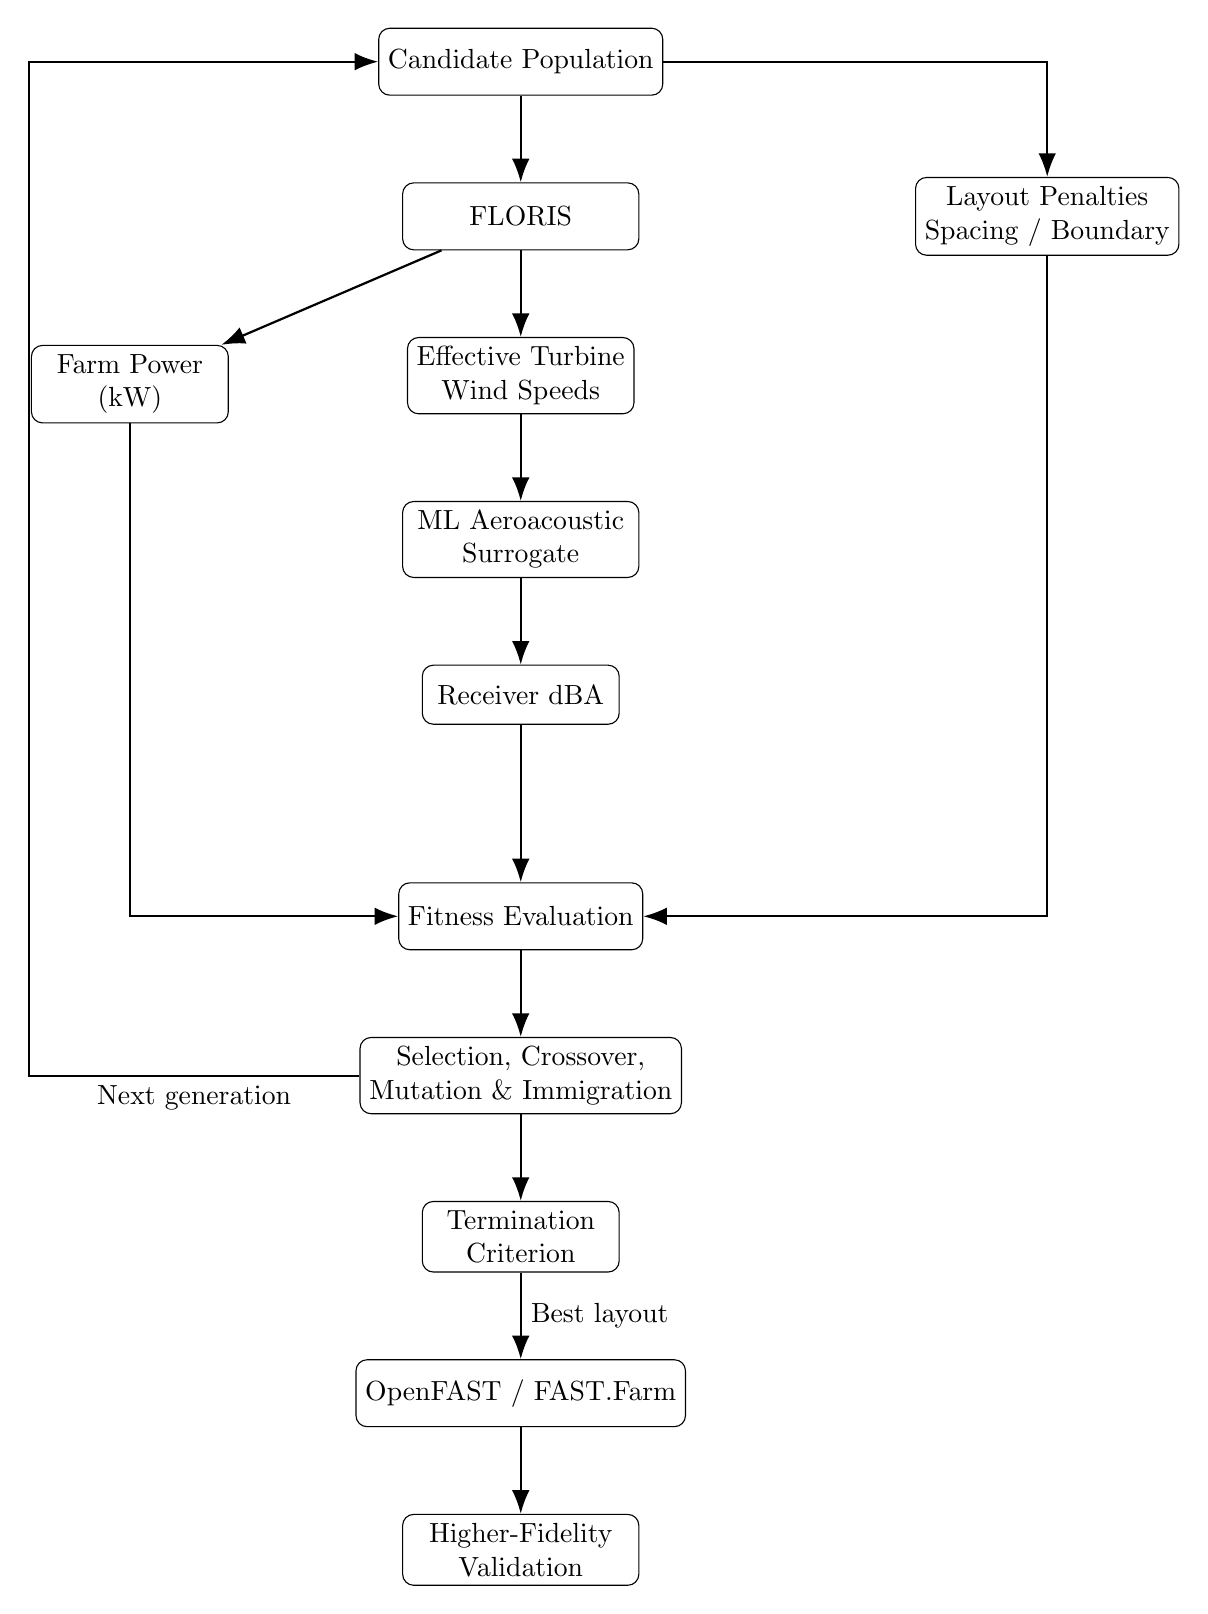
\begin{tikzpicture}[
        node distance=1.1cm and 2.0cm,
        box/.style={
            rectangle,
            draw,
            rounded corners,
            align=center,
            minimum width=3.0cm,
            minimum height=0.85cm
        },
        smallbox/.style={
            rectangle,
            draw,
            rounded corners,
            align=center,
            minimum width=2.5cm,
            minimum height=0.75cm
        },
        arrow/.style={
            -{Latex[length=3mm]},
            thick
        }
    ]

    % --------------------------------------------------------
    % Main optimization flow
    % --------------------------------------------------------

    \node[box] (population)
        {Candidate Population};

    \node[box, below=of population] (floris)
        {FLORIS};

    % FLORIS branches
    \node[smallbox, below left=1.2cm and 2.2cm of floris] (power)
        {Farm Power\\(kW)};

    \node[smallbox, below=of floris] (velocity)
        {Effective Turbine\\Wind Speeds};

    \node[box, below=of velocity] (aa)
        {ML Aeroacoustic\\Surrogate};

    \node[smallbox, below=of aa] (dba)
        {Receiver dBA};

    % Layout penalties branch
    \node[box, right=3.5cm of floris] (penalties)
        {Layout Penalties\\
        Spacing / Boundary};

    % Fitness
    \node[box, below=2.0cm of dba] (fitness)
        {Fitness Evaluation};

    % Genetic operations
    \node[box, below=of fitness] (operators)
        {Selection, Crossover,\\
        Mutation \& Immigration};

    % Termination
    \node[smallbox, below=of operators] (termination)
        {Termination\\Criterion};

    \node[box, below=of termination] (openfast)
        {OpenFAST / FAST.Farm};

    \node[box, below=of openfast] (validation)
        {Higher-Fidelity\\Validation};


    % --------------------------------------------------------
    % Arrows
    % --------------------------------------------------------

    % Population -> FLORIS
    \draw[arrow]
        (population) -- (floris);

    % Population -> layout penalties
    \draw[arrow]
        (population.east)
        -|
        (penalties.north);

    % FLORIS branches
    \draw[arrow]
        (floris)
        -- (power);

    \draw[arrow]
        (floris)
        -- (velocity);

    % Velocity -> AA -> dBA
    \draw[arrow]
        (velocity)
        -- (aa);

    \draw[arrow]
        (aa)
        -- (dba);

    % Power -> fitness
    \draw[arrow]
        (power.south)
        |- (fitness.west);

    % dBA -> fitness
    \draw[arrow]
        (dba)
        -- (fitness);

    % Layout penalties -> fitness
    \draw[arrow]
        (penalties.south)
        |- (fitness.east);

    % Fitness -> genetic operators
    \draw[arrow]
        (fitness)
        -- (operators);

    % Operators -> termination
    \draw[arrow]
        (operators)
        -- (termination);

    % Termination -> OpenFAST
    \draw[arrow]
        (termination)
        -- node[right] {Best layout}
        (openfast);

    % OpenFAST -> validation
    \draw[arrow]
        (openfast)
        -- (validation);


    % --------------------------------------------------------
    % Next-generation loop
    % --------------------------------------------------------

    \coordinate (loopLeft)
        at ($(operators.west)+(-4.2cm,0)$);

    \coordinate (loopTop)
        at ($(population.west)+(-1.2cm,0)$);

    \draw[arrow]
        (operators.west)
        -- node[below] {Next generation}
        (loopLeft)
        |- (loopTop)
        -- (population.west);

    \end{tikzpicture}

    \caption{
        Overall genetic-algorithm optimization and
        OpenFAST/FAST.Farm validation workflow.
    }
    \label{fig:overall-workflow}

\end{figure}

\subsection{Aeroacoustic Surrogate Model}



\subsubsection{Aeroacoustic Training Data}

The training data for the aeroacoustic surrogate were generated using
single-turbine OpenFAST simulations. Because each turbine was simulated
independently, wake interactions between turbines were not included in
the training-data generation process. Wake effects are instead accounted
for later in the optimization workflow using FLORIS, which provides the
effective wind speed experienced by each turbine.

Two primary variables were varied when generating the aeroacoustic
training data: turbine wind speed and the position of the acoustic
observer relative to the turbine. The wind-speed range was sampled from
3.0 to 24.5~m/s in increments of 0.5~m/s,

\begin{equation}
    v \in \{3.0, 3.5, 4.0, \ldots, 24.5\},
\end{equation}

resulting in 44 distinct wind-speed conditions.

Observer locations were defined in polar coordinates using radial
distance $r$ and azimuth angle $\theta$. Twenty radial distances were
generated using logarithmic spacing between 100 and 1000~m. A reference
radius of 200~m was additionally included to provide a higher-resolution
angular sampling at a representative observer distance. Each of the
logarithmically spaced radii was evaluated at 16 azimuth angles, while
the 200~m reference radius was evaluated at 32 azimuth angles.

The resulting observer sampling therefore contained

\begin{equation}
    (20 \times 16) + 32 = 352
\end{equation}

observer positions. Combining these positions with the 44 wind-speed
conditions produced a total of

\begin{equation}
    N_{\mathrm{samples}}
    = 44 \times 352
    = 15{,}488
\end{equation}

single-turbine aeroacoustic training samples.

Table~\ref{tab:aa-training-data} summarizes the sampling strategy.

\begin{table}[htbp]
    \centering
    \caption{OpenFAST aeroacoustic training-data sampling.}
    \label{tab:aa-training-data}

    \begin{tabular}{lll}
        \toprule
        Variable & Sampling & Number of Values \\
        \midrule
        Wind speed $v$
            & 3.0--24.5~m/s, 0.5~m/s increments
            & 44 \\

        Radial distance $r$
            & Logarithmically spaced, 100--1000~m
            & 20 \\

        Azimuth $\theta$
            & 16 angles per logarithmically spaced radius
            & 16 \\

        Reference radius
            & 200~m with 32 azimuth angles
            & 32 observer positions \\
        \midrule
        Total observer positions
            & $(20 \times 16) + 32$
            & 352 \\

        Total training samples
            & $44 \times 352$
            & 15,488 \\
        \bottomrule
    \end{tabular}
\end{table}

\begin{figure}[htbp]
    \centering

    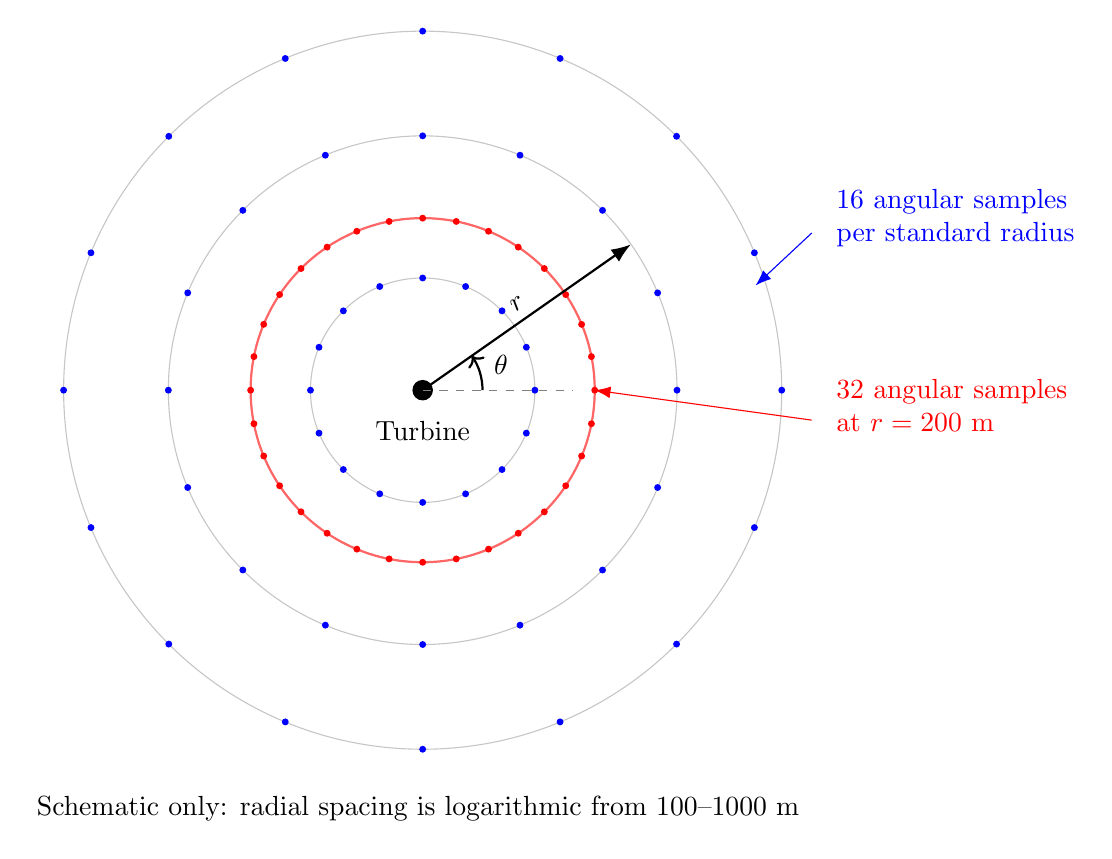
\begin{tikzpicture}[
        scale=0.95,
        turbine/.style={
            circle,
            draw,
            fill=black,
            minimum size=7pt,
            inner sep=0pt
        },
        normalobs/.style={
            circle,
            fill=blue,
            minimum size=2.5pt,
            inner sep=0pt
        },
        denseobs/.style={
            circle,
            fill=red,
            minimum size=2.5pt,
            inner sep=0pt
        }
    ]

    % --------------------------------------------------------
    % Representative radial rings
    % --------------------------------------------------------

    \def\radii{1.5,2.3,3.4,4.8}

    \foreach \r in \radii {
        \draw[
            gray!45,
            thin
        ]
        (0,0) circle (\r);
    }

    % --------------------------------------------------------
    % 16 observers on representative normal rings
    % --------------------------------------------------------

    \foreach \r in {1.5,3.4,4.8} {

        \foreach \angle in {
            0,22.5,45,67.5,
            90,112.5,135,157.5,
            180,202.5,225,247.5,
            270,292.5,315,337.5
        } {

            \node[
                normalobs
            ]
            at (
                \angle:\r
            ) {};

        }
    }

    % --------------------------------------------------------
    % Dense 200 m reference ring
    % --------------------------------------------------------

    \draw[
        red!60,
        thick
    ]
    (0,0) circle (2.3);

    \foreach \angle in {
        0,11.25,22.5,33.75,
        45,56.25,67.5,78.75,
        90,101.25,112.5,123.75,
        135,146.25,157.5,168.75,
        180,191.25,202.5,213.75,
        225,236.25,247.5,258.75,
        270,281.25,292.5,303.75,
        315,326.25,337.5,348.75
    } {

        \node[
            denseobs
        ]
        at (
            \angle:2.3
        ) {};

    }

    % --------------------------------------------------------
    % Turbine
    % --------------------------------------------------------

    \node[
        turbine
    ]
    (turbine)
    at (0,0) {};

    \node[
        below=4pt of turbine
    ]
    {Turbine};

    % --------------------------------------------------------
    % Radius marker
    % --------------------------------------------------------

    \draw[
        -{Latex[length=2.5mm]},
        thick
    ]
    (0,0)
    -- node[
        above,
        sloped
    ] {$r$}
    (35:3.4);

    % --------------------------------------------------------
    % Angle marker
    % --------------------------------------------------------

    \draw[
        gray,
        dashed
    ]
    (0,0)
    -- (2.0,0);

    \draw[
        ->,
        thick
    ]
    (0.8,0)
    arc[
        start angle=0,
        end angle=35,
        radius=0.8
    ];

    \node
    at (18:1.1)
    {$\theta$};

    % --------------------------------------------------------
    % Labels
    % --------------------------------------------------------

    \node[
        blue,
        align=left,
        anchor=west
    ]
    at (5.4,2.3)
    {16 angular samples\\per standard radius};

    \draw[
        blue,
        -{Latex[length=2mm]}
    ]
    (5.2,2.1)
    -- (4.45,1.4);

    \node[
        red,
        align=left,
        anchor=west
    ]
    at (5.4,-0.2)
    {32 angular samples\\at $r=200$ m};

    \draw[
        red,
        -{Latex[length=2mm]}
    ]
    (5.2,-0.4)
    -- (2.3,0);

    % --------------------------------------------------------
    % Scale annotation
    % --------------------------------------------------------

    \node[
        align=center
    ]
    at (0,-5.6)
    {
        Schematic only:
        radial spacing is logarithmic from 100--1000 m
    };

    \end{tikzpicture}

    \caption{
        Schematic representation of the observer sampling used to generate
        the single-turbine aeroacoustic training dataset. Standard radial
        distances use 16 uniformly distributed azimuth angles, while the
        200~m reference radius uses a denser 32-angle sampling.
    }

    \label{fig:aa-training-geometry}

\end{figure}


\subsubsection{Candidate Feature Representations}

The data generated from the OpenFAST simulations initially contained
three input variables: wind speed $v$, relative observer coordinate $X$,
and relative observer coordinate $Y$. Although the Cartesian coordinates
fully describe the observer location, the aeroacoustic field exhibits a
strong radial and directional structure. Several alternative feature
representations were therefore evaluated to make this underlying geometry
more explicit to the machine-learning models.

The relative Cartesian coordinates were first transformed into polar
coordinates according to

\begin{equation}
    r = \sqrt{X^2 + Y^2},
\end{equation}

and

\begin{equation}
    \theta = \operatorname{atan2}(Y,X).
\end{equation}

Directly using $\theta$ as a numerical feature introduces an artificial
discontinuity at the angular boundary. For example, directions immediately
below $2\pi$ and immediately above $0$ are physically adjacent but
numerically distant. To preserve the periodic nature of the observer
azimuth, the angular coordinate was therefore encoded using

\begin{equation}
    c_{\theta} = \cos(\theta),
    \qquad
    s_{\theta} = \sin(\theta).
\end{equation}

Distance was also represented using several transformations. Under
geometric spreading, acoustic intensity decreases with increasing
distance, while sound-pressure level is expressed on a logarithmic scale.
A logarithmic transformation of the observer distance,

\begin{equation}
    r_{\log} = \log_{10}(r),
\end{equation}

was therefore evaluated as a candidate feature. Reciprocal distance terms
were additionally considered,

\begin{equation}
    r^{-1} = \frac{1}{r},
    \qquad
    r^{-2} = \frac{1}{r^2},
\end{equation}

to determine whether explicitly representing distance-decay relationships
improved predictive performance.

Rather than selecting one representation a priori, five candidate feature
sets were constructed and evaluated with each candidate machine-learning
model. These feature sets are summarized in
Table~\ref{tab:feature-sets}. The complete set of original and engineered
features is retained in \texttt{training\_data.csv}.

\begin{table}[htbp]
    \centering
    \caption{Candidate feature representations evaluated for the
    aeroacoustic surrogate.}
    \label{tab:feature-sets}

    \begin{tabularx}{\textwidth}{
        >{\raggedright\arraybackslash}p{0.22\textwidth}
        >{\raggedright\arraybackslash}X
        >{\raggedright\arraybackslash}X
    }
        \toprule
        \textbf{Feature Set} &
        \textbf{Input Features} &
        \textbf{Purpose} \\
        \midrule

        Cartesian
        & $v,\ X,\ Y$
        & Original spatial representation \\

        Polar
        & $v,\ r,\ \cos\theta,\ \sin\theta$
        & Explicit radial and directional representation \\

        Polar + log distance
        & $v,\ \log_{10}(r),\ \cos\theta,\ \sin\theta$
        & Logarithmic distance representation \\

        Polar + raw/log distance
        & $v,\ r,\ \log_{10}(r),\ \cos\theta,\ \sin\theta$
        & Combined raw and logarithmic distance \\

        Polar + distance decay
        & $v,\ \log_{10}(r),\ r^{-1},\ r^{-2},\
          \cos\theta,\ \sin\theta$
        & Multiple representations of distance decay \\

        \bottomrule
    \end{tabularx}
\end{table}

The feature representation was not selected independently of the
regression model. Instead, each candidate machine-learning algorithm was
trained and evaluated using all five feature sets. The final combination
of model architecture and feature representation was selected based on
predictive performance, as described in the following section.

\subsubsection{Model Training and Selection}

\lipsum[12]

\subsubsection{Final Surrogate Implementation}

The machine-learning surrogate uses the input feature vector

\begin{equation}
    \mathbf{x}
    =
    \begin{bmatrix}
        v &
        \log_{10}(r) &
        \cos(\theta) &
        \sin(\theta)
    \end{bmatrix}.
\end{equation}

The surrogate then approximates the relationship

\begin{equation}
    \hat{L}_{A}
    =
    f\left(
        v,
        \log_{10}(r),
        \cos(\theta),
        \sin(\theta)
    \right),
\end{equation}

where $\hat{L}_{A}$ is the predicted A-weighted sound level.

\subsubsection{Aeroacoustic Aggregation}

Independent turbine noise contributions are combined in the
linear acoustic-energy domain:

\begin{equation}
    L_{\mathrm{total}}
    =
    10 \log_{10}
    \left(
        \sum_{i=1}^{N}
        10^{L_i/10}
    \right).
\end{equation}

Time-varying sound levels may similarly be reduced using

\begin{equation}
    L_{\mathrm{eq}}
    =
    10 \log_{10}
    \left(
        \frac{1}{T}
        \sum_{t=1}^{T}
        10^{L_t/10}
    \right).
\end{equation}

\subsection{Genetic Algorithm}

\lipsum[13]

\subsubsection{Chromosome Representation and Initialization}

\subsubsection{Fitness Function}

The optimization objective can be expressed generally as

\begin{equation}
    F =
    P_{\mathrm{expected}}
    - C_{\mathrm{spacing}}
    - C_{\mathrm{noise}}
    - C_{\mathrm{boundary}},
\end{equation}

where $P_{\mathrm{expected}}$ represents expected farm power and
the remaining terms represent constraint penalties.


\subsubsection{Wind Scenarios}

\lipsum[14]

\subsubsection{Genetic Operators}

\lipsum[14]




\subsection{OpenFAST Validation}

\lipsum[15]


% ============================================================
% 4. Results
% ============================================================

\section{Results}

\subsection{Surrogate Model Performance}

\lipsum[16]

An example results table is shown in
Table~\ref{tab:model-performance}.

\begin{table}[htbp]
    \centering
    \caption{Example surrogate model performance.}
    \label{tab:model-performance}

    \begin{tabular}{lccc}
        \toprule
        Model & MAE (dBA) & RMSE (dBA) & $R^2$ \\
        \midrule
        Model A & 0.10 & 0.15 & 0.999 \\
        Model B & 0.15 & 0.22 & 0.997 \\
        Model C & 0.20 & 0.28 & 0.995 \\
        \bottomrule
    \end{tabular}
\end{table}


\subsection{Genetic Algorithm Performance}

\lipsum[17]


\subsection{Optimized Layout}

\lipsum[18]


\subsection{OpenFAST Validation}

\lipsum[19]


% ============================================================
% 5. Discussion
% ============================================================

\section{Discussion}

\lipsum[20-21]


% ============================================================
% 6. Limitations
% ============================================================

\section{Limitations}

\lipsum[22]

Example limitations could be presented as:

\begin{itemize}

    \item OpenFAST validation currently uses deterministic
    uniform inflow.

    \item The aeroacoustic surrogate is valid only within the
    domain represented by its training data.

    \item The Genetic Algorithm does not guarantee identification
    of the global optimum.

    \item Additional turbulence conditions would require further
    high-fidelity simulations.

\end{itemize}


% ============================================================
% 7. Future Work
% ============================================================

\section{Future Work}

\lipsum[23]


% ============================================================
% 8. Conclusion
% ============================================================

\section{Conclusion}

\lipsum[24]


% ============================================================
% References
% ============================================================

\begin{thebibliography}{9}

\bibitem{openfast}
Author,
\textit{Example OpenFAST Reference},
Publisher or Journal,
Year.

\bibitem{floris}
Author,
\textit{Example FLORIS Reference},
Publisher or Journal,
Year.

\end{thebibliography}


% ============================================================
% Appendix
% ============================================================

\appendix

\section{Optimization Parameters}

\lipsum[25]

\section{Additional Results}

\lipsum[26]


\end{document}